\section{System Architecture}

The system can operate in one of two modes. In local mode, the simulation runs in one process with a
scenario defined in code. The remote mode is described below.

\subsection{Distributed Architecture}

\begin{figure*}
    \begin{center}
        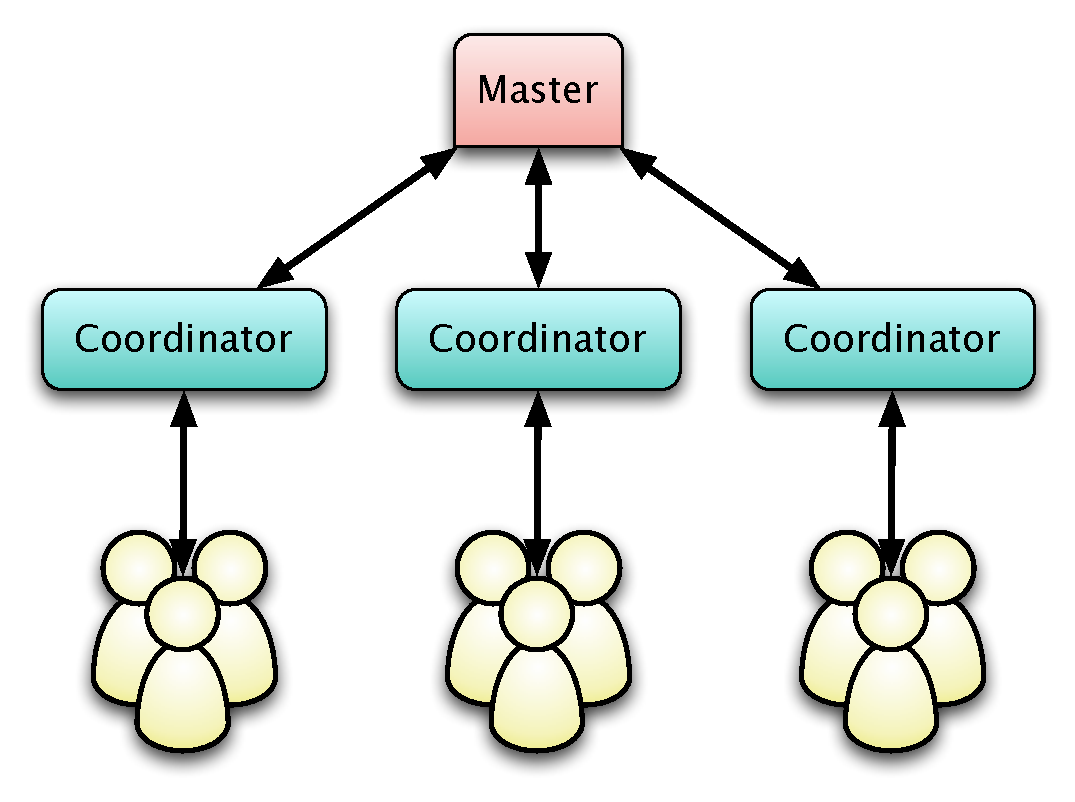
\includegraphics[width=3in]{figures/arch0.pdf}
    \end{center}
    \caption{Basic architecture of the system.}
    \label{arch}
\end{figure*}

In order to support simulations on the scale of millions of agents, Tecellate can be run in a
distributed mode on many machines. Individual components communicate via TCP. The architecture of
this distributed version is shown in figure \ref{arch}.

\begin{figure*}
    \begin{center}
        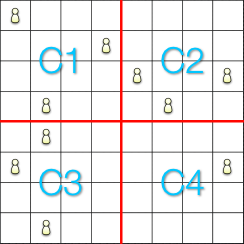
\includegraphics[width=3in]{figures/arch1.png}
    \end{center}
    \caption{Grid-based method for distributing work across coordinators}
    \label{geoarch}
\end{figure*}

Agents are run in individual processes. In order to interact with the simulation, they connect to a
\textbf{coordinator}. Coordinators are responsible for evaluating discrete grid sections each turn
and communicating their results to each other when relevant. The organization of a square grid
section is shown in figure \ref{geoarch}.

The simulation starts with all agent and coordinator processes waiting and listening at individual
addresses. A master process reads a configuration file with their addresses and initial states,
sends information about how to connect to each other, waits for the connections to finish, and
instructs the coordinators to begin the simulation. It then exits and the other processes log
simulation data to configurable log files.

Each coordinator is responsible for a rectangular section of the grid. These sections are assigned
at the start of the simulation and do not change. Coordinators are connected with neighbor
coordinators that share adjacent grid sections. When an agent moves from one grid section to
another, the agent connects to the coordinator responsible for the new section.

\subsection{Coordinator Implementation Details}

There are two main types of threads associated with each coordinator. One kind of thread (A-thread)
requests agent data from neighbors, and then applies the simulation rules to the agents's previous
states based on their requested actions and the states of the agents at the neighbor coordinators.
There is only one of these threads. The other kind of thread (B-thread) serves requests for agent
information from neighbors, and there is one of these for each neighbor ($|N|$).

The A-thread and the B-threads communicate using two semaphores, \textbf{turnAvailable} and
\textbf{requestsServed}. The A-thread signals \textbf{turnAvailable} $|N|$ times when a turn has
been processed, and the B-threads each wait on it before serving a new request. When a B-thread has
served a request, it signals \textbf{requestsServed}. The A-thread waits on \textbf{requestsServed}
before it begins processing a new turn to avoid overwriting data that B-threads are still serving.
The system starts with \textbf{turnAvailable} unlocked for the B-threads.

This system allows processing and RPC serving to run in parallel, with processing running one step
ahead of RPC serving.

Processing a turn (in the A-thread) involves exchanging messages with each agent to get its moves
for the next turn. This may happen over TCP or in-memory communication channels depending on the
mode of operation.

\subsection{Issues and Possible Improvements}

The biggest issue with the current implementation is that distributed communication via TCP is
orders of magnitude slower than communication in memory. While this limiation is not surprising, it
is probably possible to improve communication speed by switching to a UDP-based protocol.

The application is highly multithreaded even within individual components. A modest run will have 40
or more threads. These are not OS-level threads but rather lightweight runtime-level threads.
Despite their lightweight nature, a large proportion are waiting for input most of the time, for
example to serve an RPC request. Our educated guess is that 60\% of threads are in this state at any
given moment. These threads may be wasting more CPU cycles than necessary when they are scheduled.

Performance improves when the language runtime is instructed to split the threads across multiple
CPU cores, but when this is done, a major memory leak manifests which makes the system unusable.
This memory leak may be caused by the language runtime, but we are still investigating the issue.

If agents cluster in one geographic area, one coordinator may have a significantly higher burden
than the others. This problem could be solved by allowing the master process to dynamically
reallocate the space assigned to each coordinator. This dynamic reassignment is very similar
to the problem of assigning many application instances to many servers, but in addition to simply
trying to distribute CPU and memory load evenly, we are also trying keep traffic between coordinators to a minimum. It would take another paper to describe an effective algorithm to accomplish this goal, and probably a simulator-simulator to test it.
